\documentclass[12pt]{article}
\usepackage[utf8]{inputenc}
\usepackage[T1]{fontenc}
\usepackage{geometry}
\usepackage{graphicx}
\usepackage{makeidx}
\geometry{margin=2.5cm}
\usepackage{fancyhdr}

\begin{document}
	
	\thispagestyle{empty}
	
	\begin{center}
		
\includegraphics[width=3.1cm,height=2cm]{logo}\\
		UNIVERSIDAD SIMÓN BOLÍVAR\\
		DEPARTAMENTO DE ELECTRÓNICA Y CIRCUITOS\\
		EC1281 - LABORATORIO DE MEDICIONES ELÉCTRICAS\\
		SECCIÓN 1 - GRUPO 1\\
		
		\vspace{7cm}
		\textbf{\Large INFORME - PRÁCTICA \#7}\\
		INSTRUMENTO DE MEDICÓN PARA CORRIENTE ALTERNA (AC)\\
	\end{center}
	
	\begin{flushleft}
		\vspace{9cm}
		\hfill Integrantes:\\
		\hfill {\large Luis Becerra - 1910557}\\
		\hfill {\large Lorena Rojas - 1910469}\\
	\end{flushleft}
	
	\newpage
	
	\pagenumbering{Roman}
        \setcounter{page}{2}
	
	\begin{center}
		\textbf{\large RESUMEN}\\
	\end{center}
	
	En esta práctica de laboratorio, se tuvieron como objetivos principales la interpretación de las características nominales de los instrumentos de medición para corriente alterna (AC) y el uso adecuado de dichos instrumentos en mediciones en AC. Se realizaron mediciones directas e indirectas de voltajes y corrientes pico y rms, mediciones de frecuencia, desfasaje y potencia en circuitos alimentados con fuentes alternas. Además, se compararon los resultados experimentales con los valores teóricos o simulados de los circuitos. Las mediciones se llevaron a cabo utilizando voltímetros, amperímetros, multímetros y osciloscopios. Se realizaron mediciones de resistencias, voltajes pico y rms, corrientes pico, desfasaje y potencia en diferentes configuraciones de circuitos. Los resultados obtenidos fueron analizados y se concluyó sobre la precisión y confiabilidad de los instrumentos de medición utilizados.
	
	\newpage
	
	\begin{center}
		\textbf{\large ÍNDICE}\\
	\end{center}
	
	\noindent \textbf{RESUMEN} \hfill \textbf{II}\\
	\noindent \textbf{ÍNDICE} \hfill \textbf{III}\\
	\noindent \textbf{MARCO TEÓRICO} \hfill \textbf{1}\\
	\noindent \textbf{METEDOLOGÍA} \hfill \textbf{}\\
	\noindent \textbf{RESULTADOS} \hfill \textbf{}\\
	\noindent \textbf{ANÁLISIS DE RESULTADOS} \hfill \textbf{}\\
	\noindent \textbf{CONCLUSIONES} \hfill \textbf{}\\
	\noindent \textbf{BIBLIOGRAFÍA} \hfill \textbf{}\\
	\noindent \textbf{ANEXOS} \hfill \textbf{}\\
	
	\newpage
	
	\pagenumbering{arabic}
	
	\begin{center}
		\textbf{\large MARCO TEÓRICO}\\
	\end{center}
	
	\textbf{1. Valor medio cuadrático (RMS) de una señal alterna}\\
	
	El valor medio cuadrático (RMS, por sus siglas en inglés) es una medida importante para caracterizar una señal alterna. Representa el valor efectivo de la amplitud de una señal y se calcula mediante la raíz cuadrada de la media del cuadrado de los valores instantáneos de la señal a lo largo de un período.\\
	
	Para una señal periódica $V(t)$ con un período $T$, el valor RMS se define como: $$V(t) = \sqrt{\frac{1}{T}*\int_{0}^{T}V^2(t)dt}$$	
	
	Donde $V(t)$ es el valor instantáneo de la señal en un instante de tiempo $t$. El valor RMS es útil porque representa la amplitud equivalente de una señal de corriente alterna en términos de su valor continuo.\\
	
	\textbf{2. Ancho de banda de un circuito o instrumento de corriente alterna}\\
	
	El ancho de banda de un circuito o instrumento de corriente alterna se refiere al rango de frecuencias dentro del cual la respuesta del sistema es aceptablemente buena. Se define como la diferencia entre la frecuencia más alta y la frecuencia más baja que puede ser transmitida o medida por el sistema sin una degradación significativa.\\
	
	En general, el ancho de banda está relacionado con la capacidad del circuito o instrumento para responder a señales de diferentes frecuencias. Los circuitos o instrumentos con un ancho de banda amplio pueden capturar o medir señales de frecuencia más alta, mientras que aquellos con un ancho de banda más estrecho tienen una respuesta limitada a frecuencias altas.\\
	
	El ancho de banda puede estar determinado por la capacidad de los componentes del circuito, como condensadores e inductores, así como por la respuesta de los amplificadores o filtros utilizados en el sistema. Es importante considerar el ancho de banda al seleccionar un circuito o instrumento de corriente alterna para asegurarse de que pueda manejar las frecuencias de interés.\\
	
	\textbf{3. Instrumentos de medición de voltajes y corrientes AC}\\
	
	Existen varios tipos de instrumentos de medición utilizados para medir voltajes y corrientes en circuitos de corriente alterna (AC). Estos instrumentos ofrecen diferentes características y se utilizan en diferentes aplicaciones según las necesidades del usuario.
	
	\begin{itemize}
		\item \textbf{Voltímetro de AC:} Este instrumento se utiliza para medir el valor eficaz o RMS de un voltaje AC. Puede tener escalas y rangos variables para adaptarse a diferentes niveles de voltaje. Algunos voltímetros de CA también pueden medir frecuencia y desfasaje.
		
		\item \textbf{Amperímetro de AC:} Este instrumento se utiliza para medir el valor eficaz o RMS de una corriente AC. Al igual que el voltímetro de CA, puede tener escalas y rangos variables para adaptarse a diferentes niveles de corriente. Algunos amperímetros de CA también pueden medir frecuencia y desfasaje.
		
		\item \textbf{Multímetro:} Es un instrumento versátil que combina funciones de voltímetro, amperímetro y ohmímetro. Puede medir voltajes y corrientes AC en diferentes rangos, así como resistencias y otras magnitudes eléctricas. Algunos multímetros también tienen capacidades de medición de frecuencia y desfasaje.
		
		\item \textbf{Osciloscopio:} Es un instrumento utilizado para visualizar y analizar formas de onda de señales eléctricas. Puede mostrar la amplitud, frecuencia, forma de onda y desfasaje de una señal AC en una pantalla. Los osciloscopios también pueden realizar mediciones precisas de voltajes y tiempos en señales AC.
		
	\end{itemize}
	
	Cada tipo de instrumento tiene sus ventajas y limitaciones, y la elección depende del tipo de medición requerida, el rango de frecuencias de interés y la precisión necesaria.

	\newpage
	
	\begin{center}
		\textbf{\large METODOLOGÍA}\\
	\end{center}
	
	Inserte metodología
	
	\newpage
	
	\begin{center}
		\textbf{\large RESULTADOS}\\
	\end{center}
	
	A continuación se presentan los resultados obtenidos durante el trabajo en el laboratorio:
	
	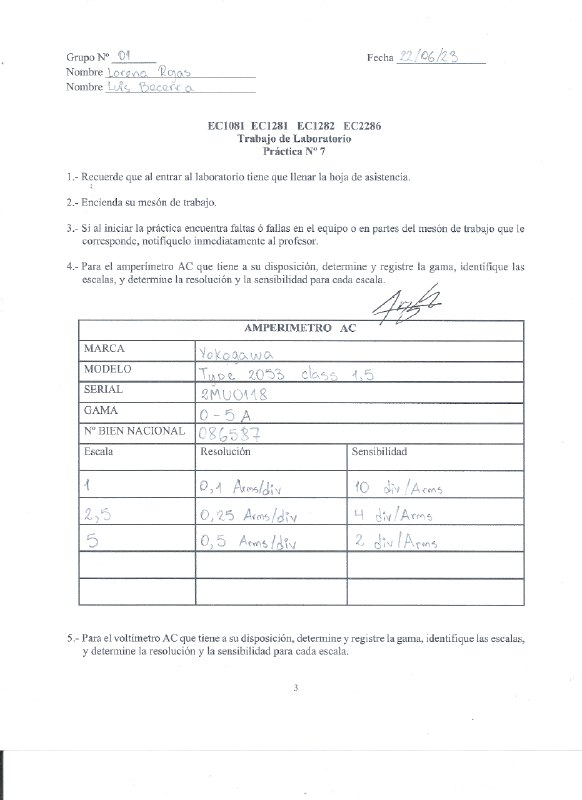
\includegraphics[width=16cm,height=21cm]{Img/Resultados_1}\\
	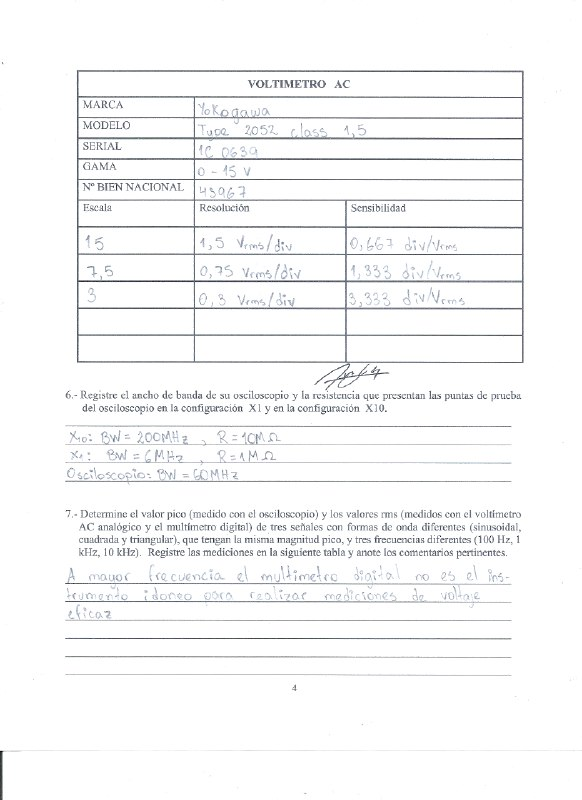
\includegraphics[width=16cm,height=21cm]{Img/Resultados_2}\\
	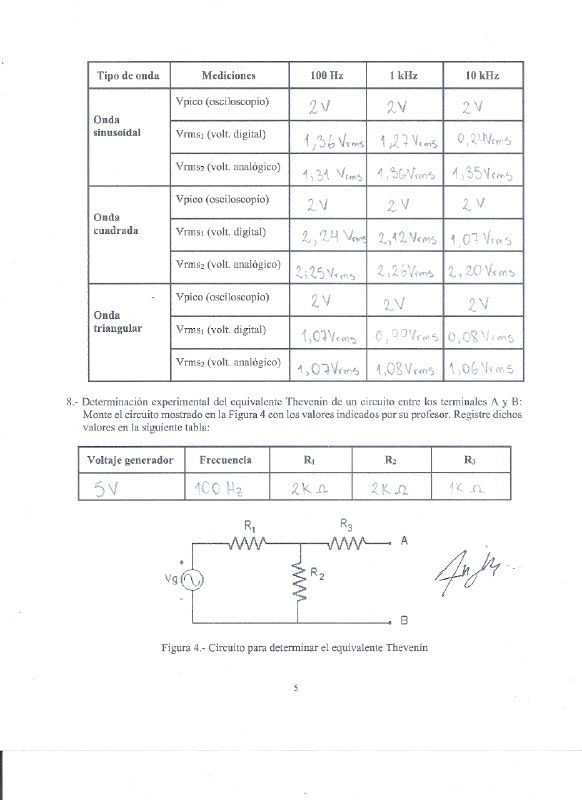
\includegraphics[width=16cm,height=21cm]{Img/Resultados_3}\\
	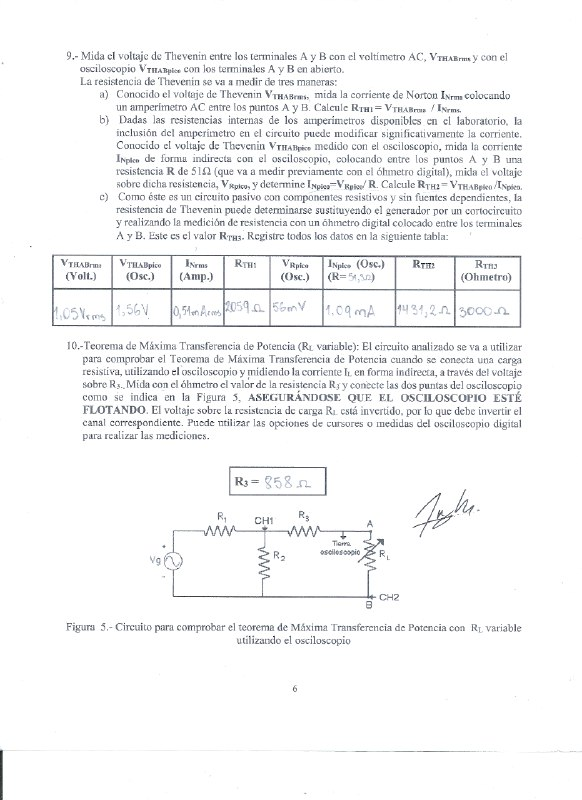
\includegraphics[width=16cm,height=21cm]{Img/Resultados_4}\\
	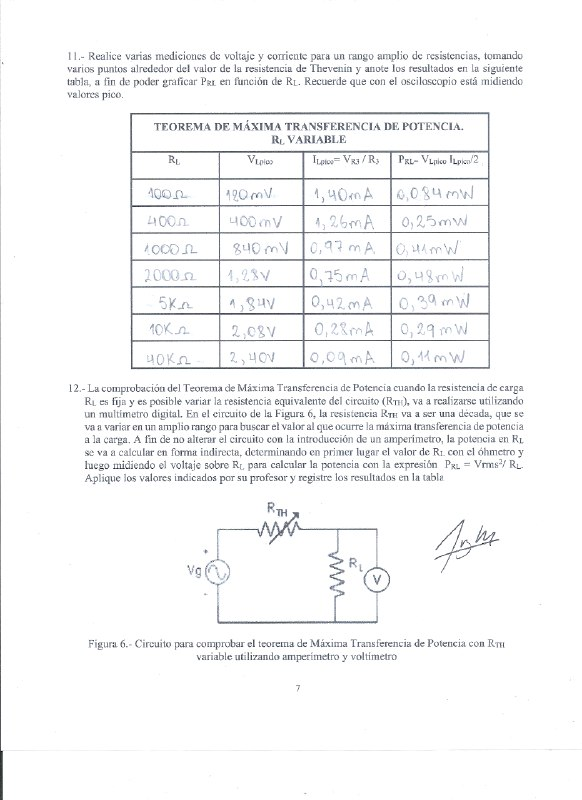
\includegraphics[width=16cm,height=21cm]{Img/Resultados_5}\\
	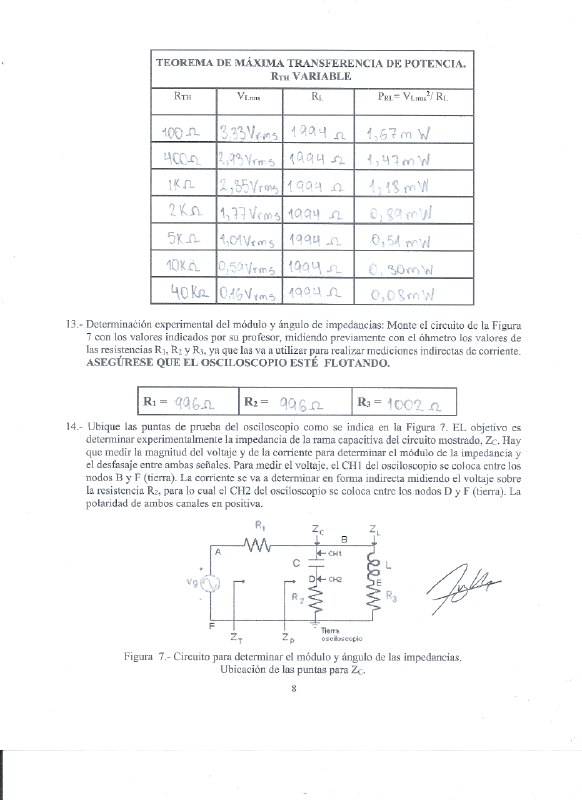
\includegraphics[width=16cm,height=21cm]{Img/Resultados_6}\\
	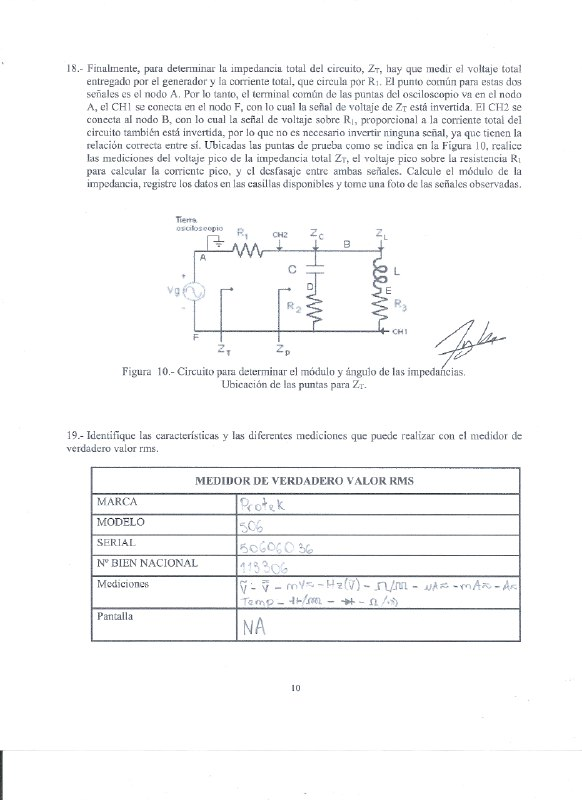
\includegraphics[width=16cm,height=21cm]{Img/Resultados_7}\\
	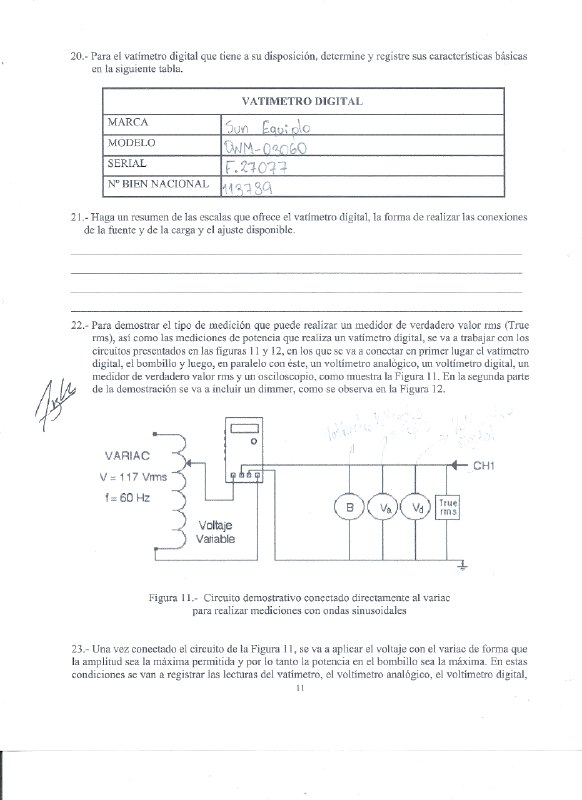
\includegraphics[width=16cm,height=21cm]{Img/Resultados_8}\\
	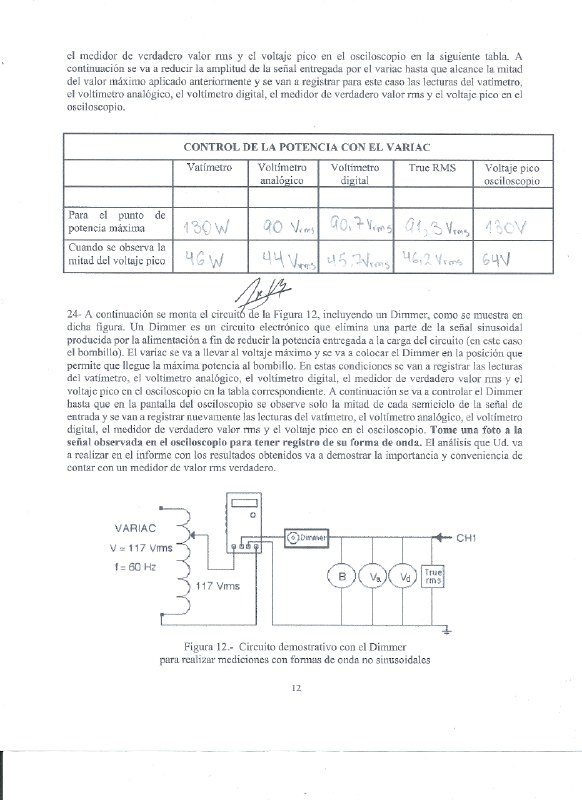
\includegraphics[width=16cm,height=21cm]{Img/Resultados_9}\\
	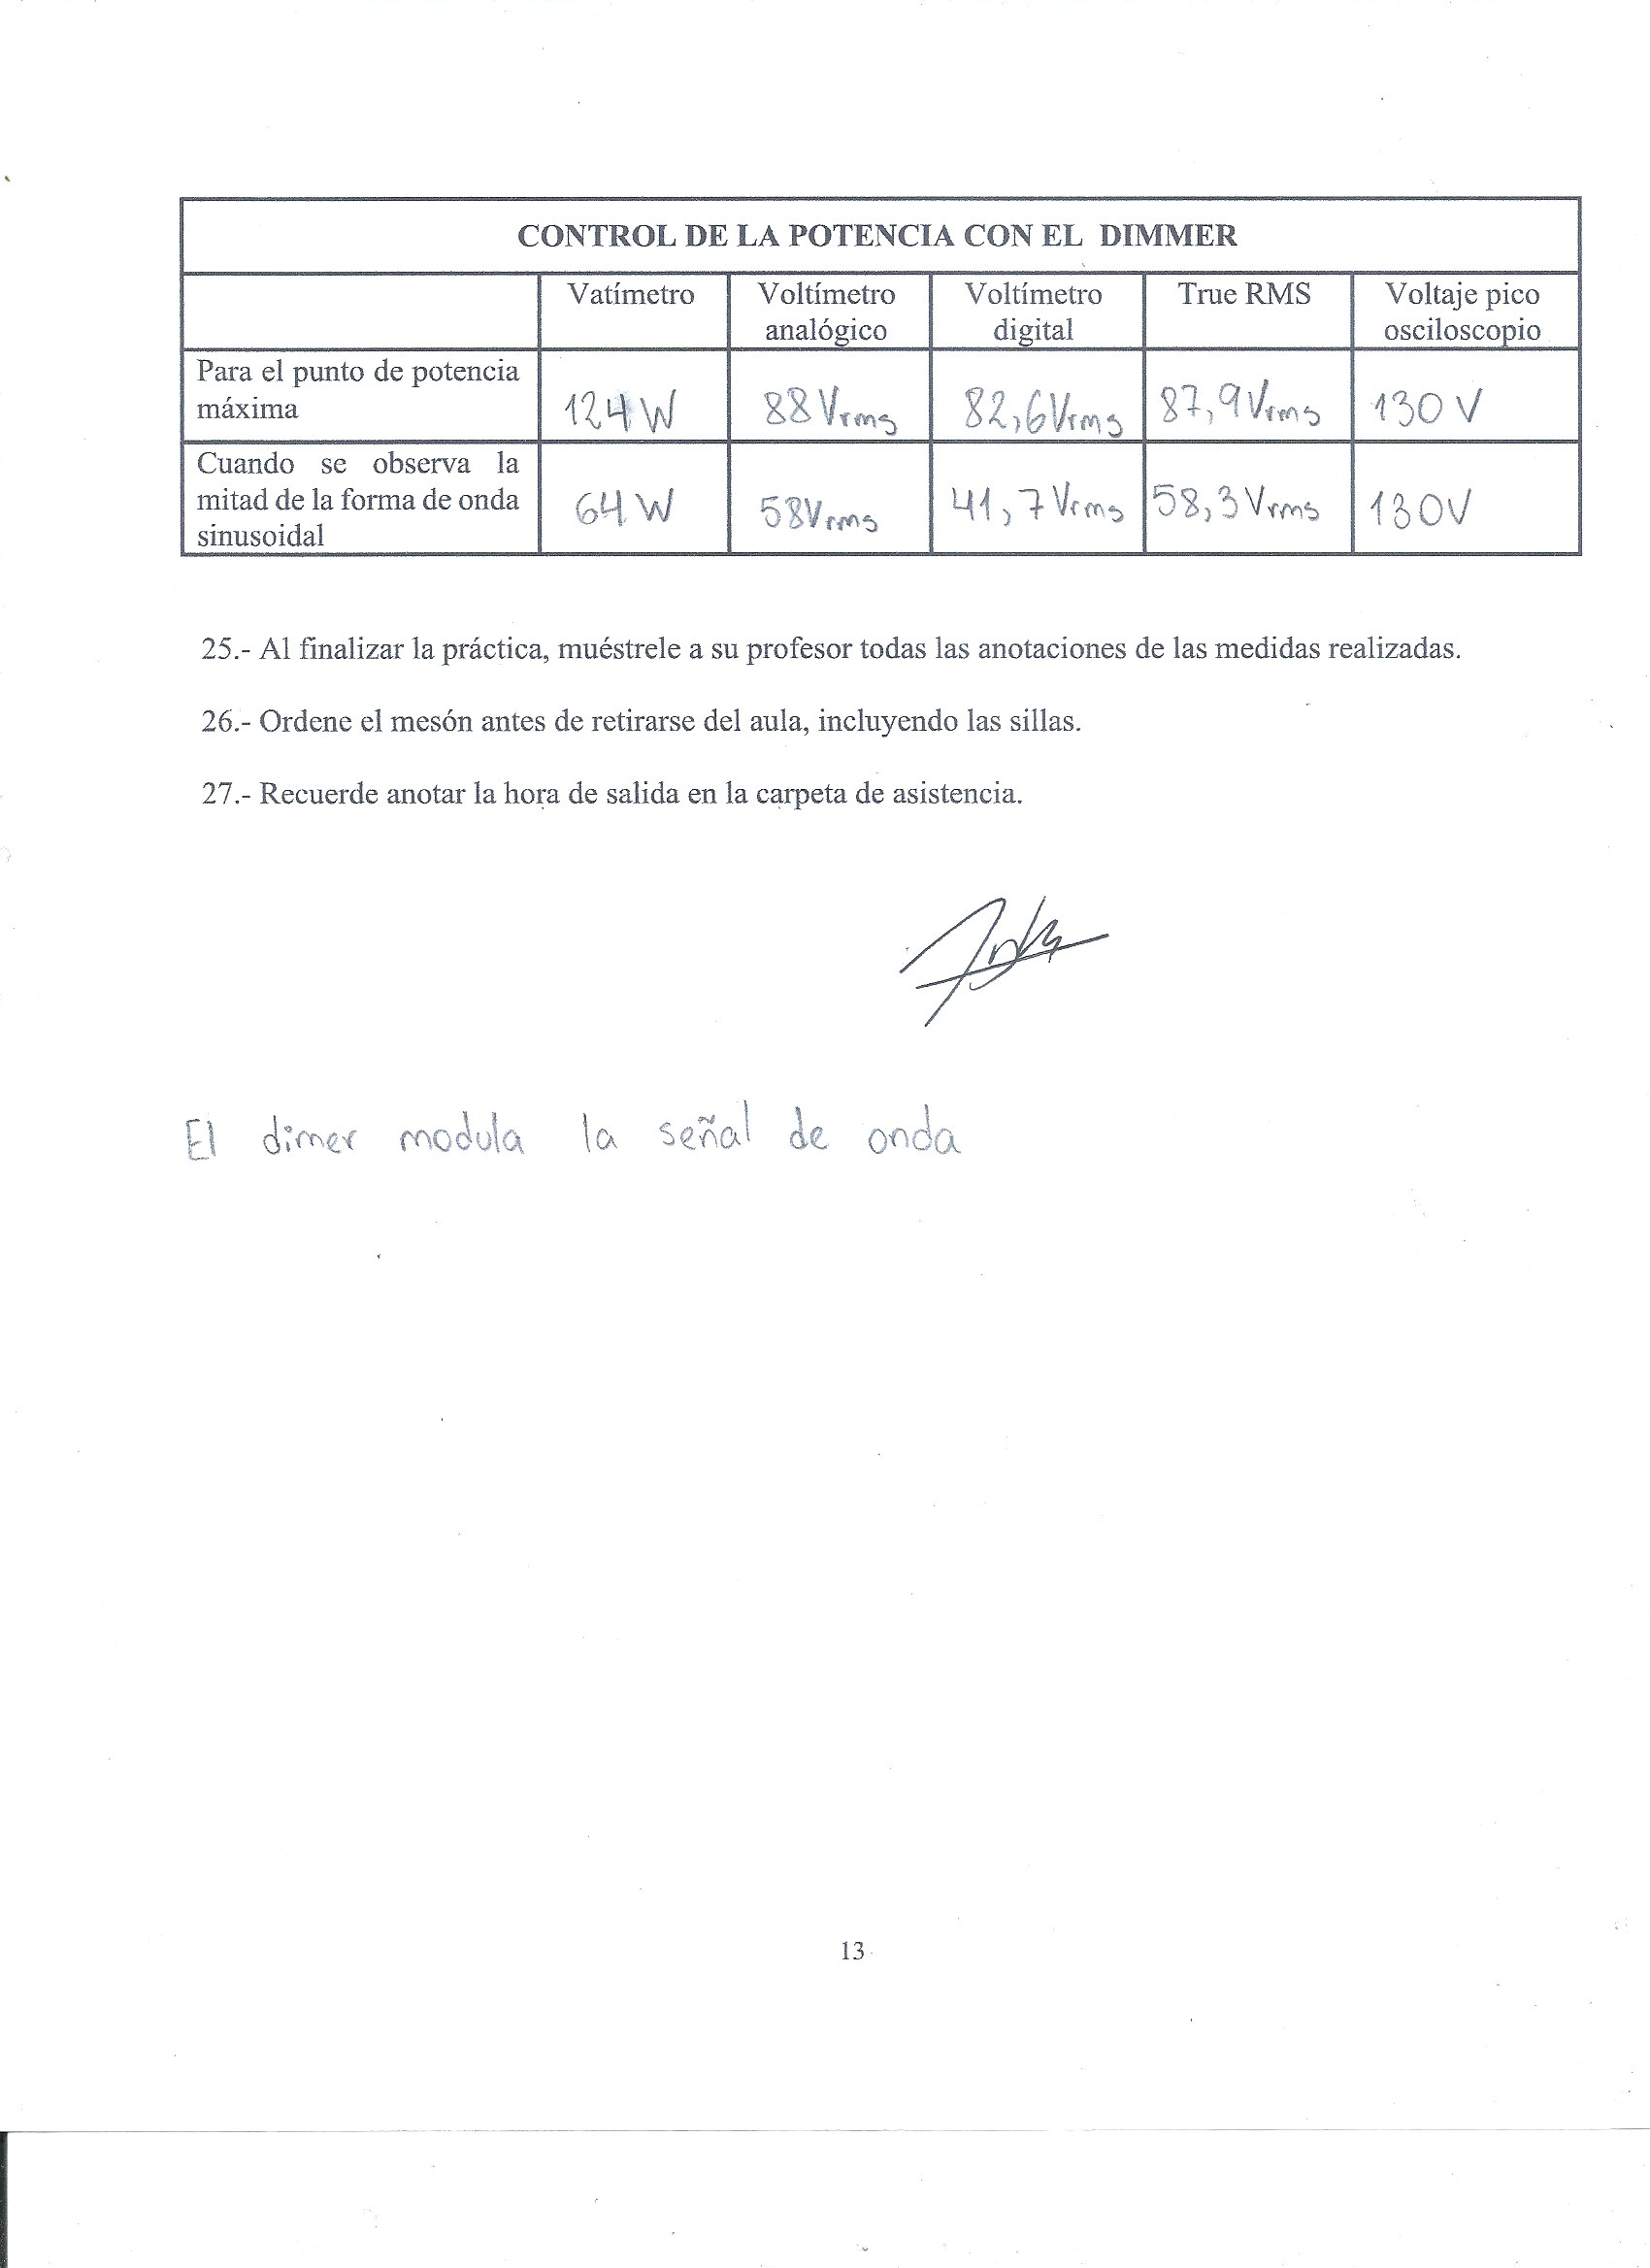
\includegraphics[width=16cm,height=21cm]{Img/Resultados_10}\\
	
	\newpage
	
	\begin{center}
		\textbf{\large ANÁLISIS DE RESULTADOS}\\
	\end{center}
	
	Inserte análisis de resultados
	
	\newpage
	
	\begin{center}
		\textbf{\large CONCLUSIONES}\\
	\end{center}
	
	Inserte conclusiones
	
	\newpage
	
	\begin{center}
		\textbf{\large BIBLIOGRAFÍA}\\
	\end{center}
	
	Inserte bibliografía
	
	\newpage
	
	\begin{center}
		\textbf{\large ANEXOS}\\
	\end{center}
	
	Inserte anexos
	
\end{document}
